
	% \section{Условия проведения эксперимента}

	% Для более объективного изучения процесса взаимодействия дискового инструмента с ПСЛО предлагается контролировать три составляющие силы резания: горизонтальную, боковую и вертикальную. Контроль этих составляющих непосредственно на рабочем органе мало эффективен, так как: требует больших трудозатрат и дорогостоящего оборудования (датчики силы, оснастка для их монтажа); невозможно изолировать влияние температуры окружающей среды, влажности, теплозапаса дорожного полотна и других факторов друг на друга; постоянно меняются физико-механические свойства ПСЛО (прочность, плотность, наличие абразивного материала). Поэтому, опираясь на работы по резанию мерзлых грунтов различными инструментами \cite{JelukevichGrunt, BaronTang, BaronShar, Zelenin}, целесообразно исследовать процесс взаимодействия полноразмерного дискового режущего инструмента с различным радиусом закругления рабочей кромки с разрушаемым массивом путем стендовых испытаний в лабораторных условиях.
	
	% В качестве режущего инструмента принят заостренный дисковый	резец изображенный на рисунке \ref{fig:DRI}. 
	% \begin{figure}[ht]
	% 	\centering
	% 	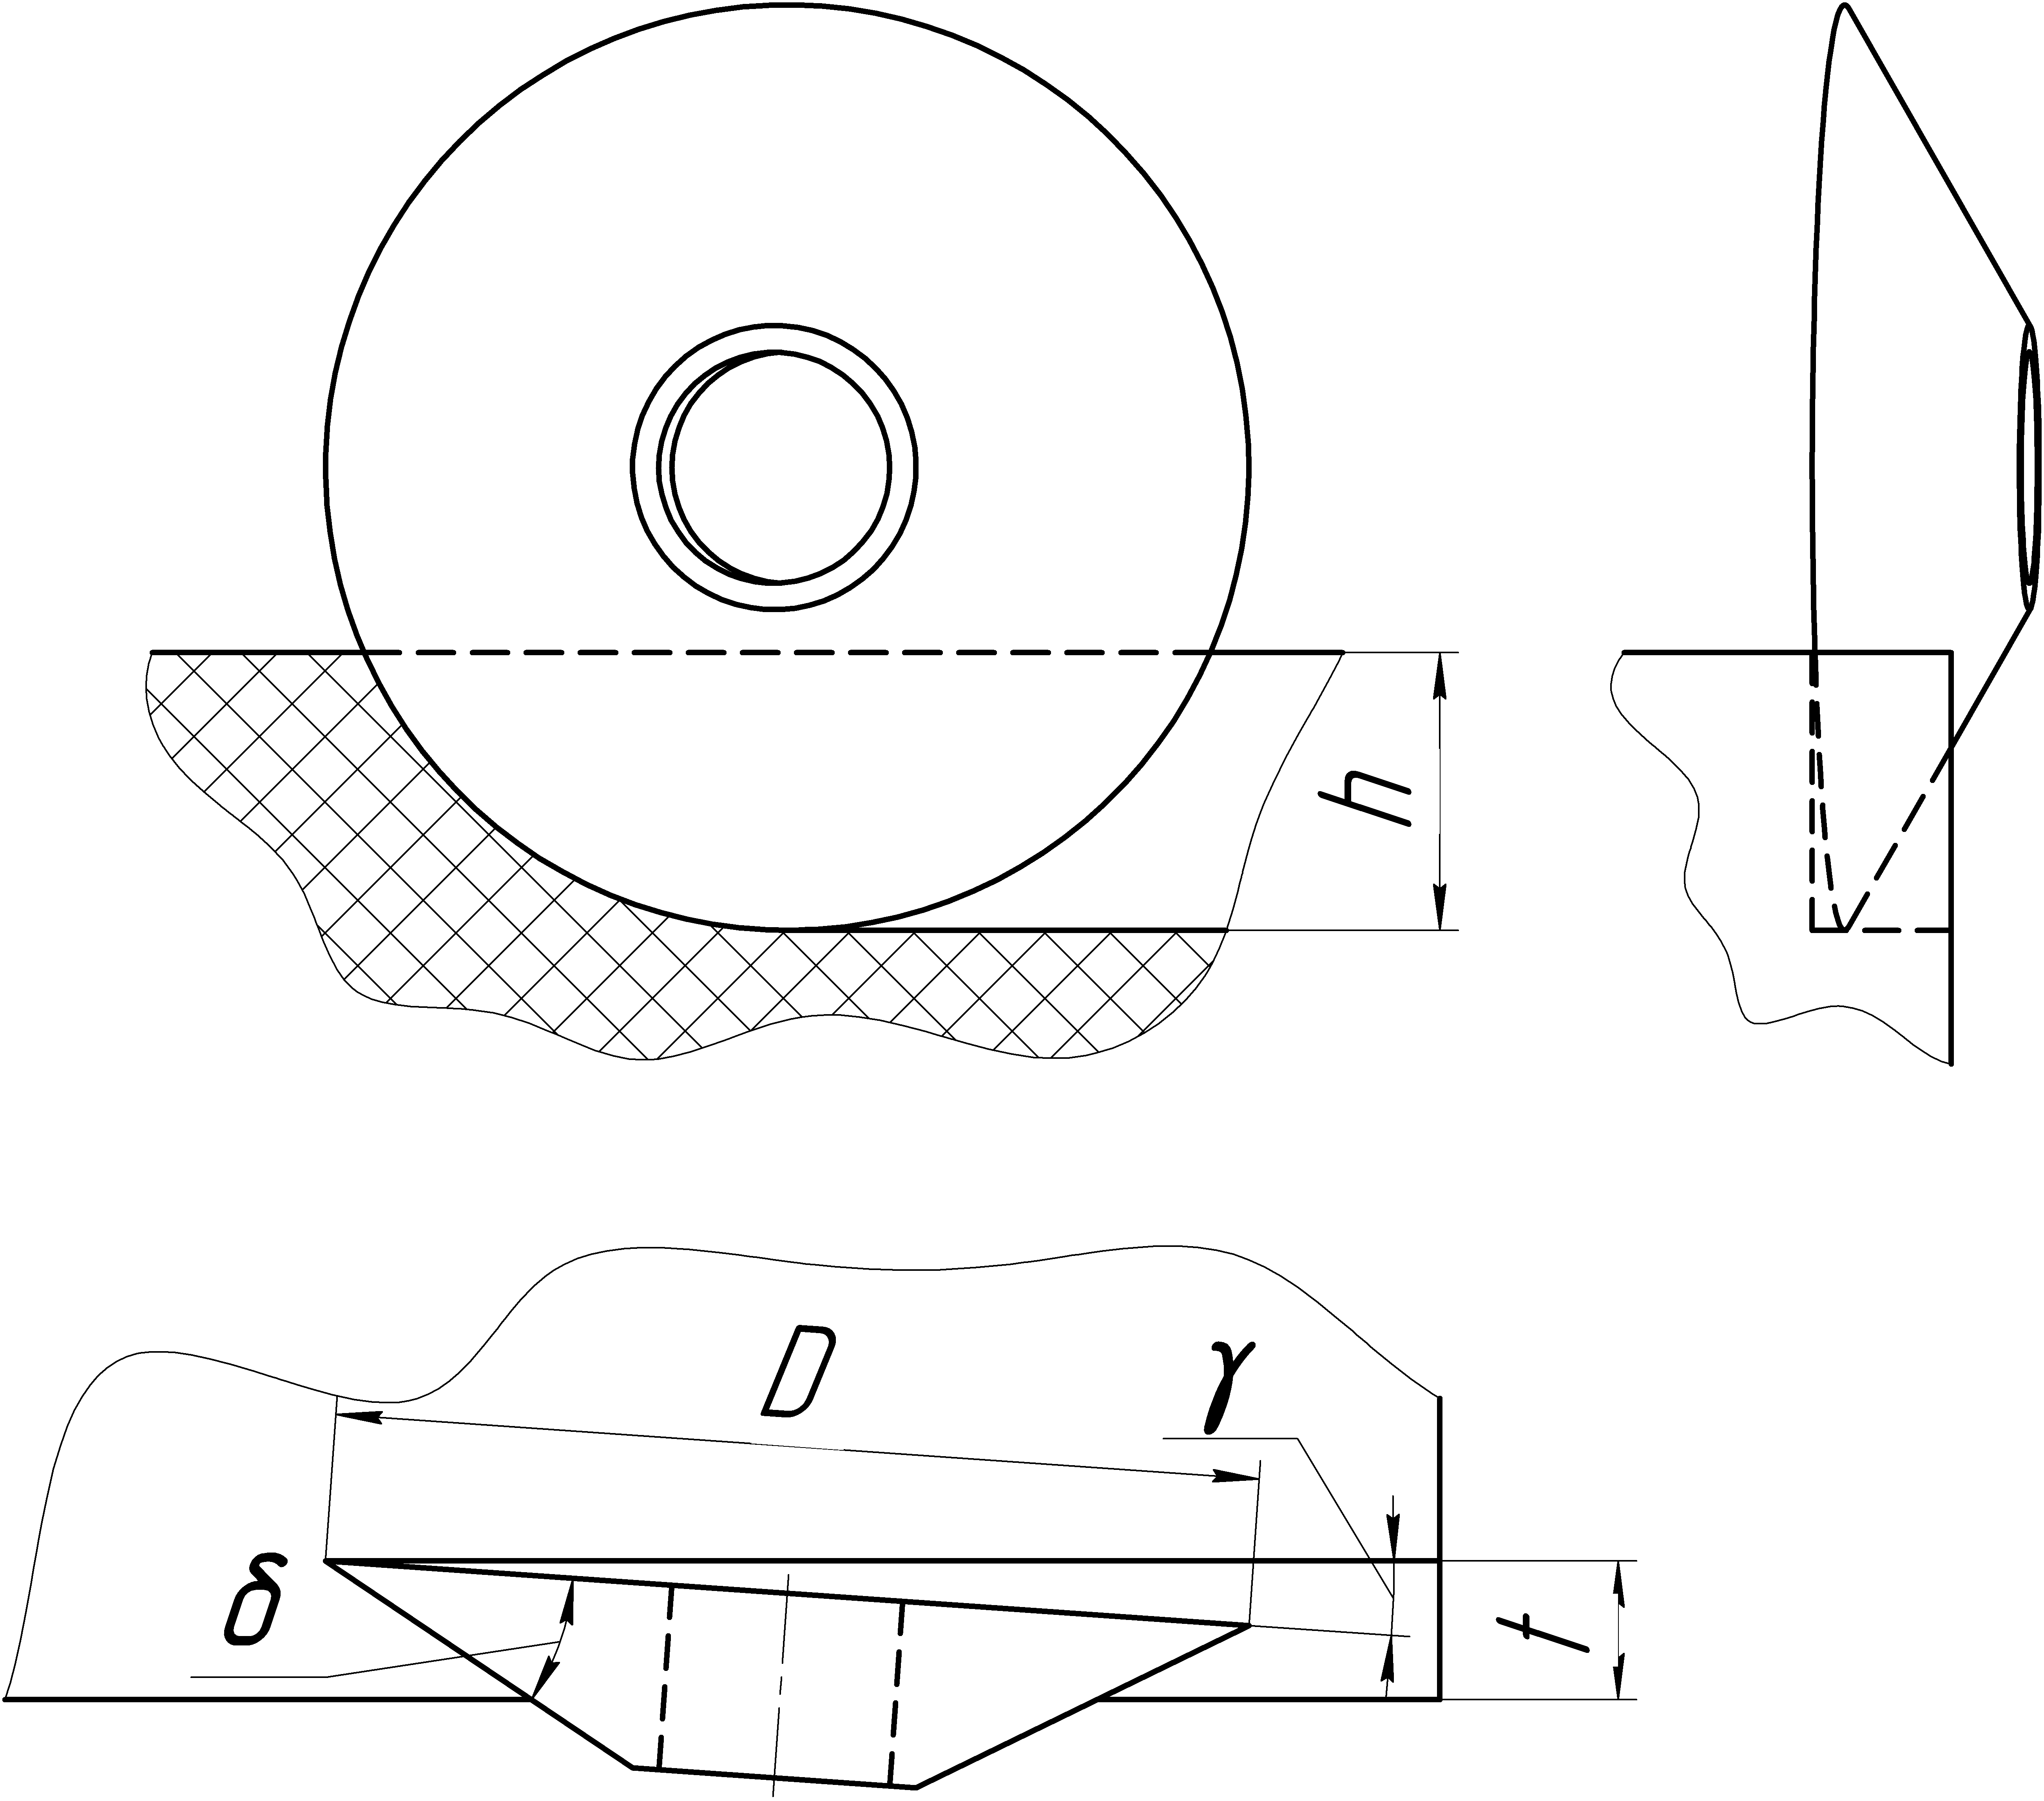
\includegraphics[width=0.5\textwidth]{DRI}

	% 	$t$ "--- шаг резания; $D$ "--- диаметр дискового резца; $\delta$ "--- угол заострения; $h$ "--- глубина резания; $\gamma$ "--- задний угол. 
	% 	\caption{Схема взаимодействия дискового режущего инструмента с разрушаемым массивом} 
	% 	\label{fig:DRI}  
	% \end{figure}

	% При проведении экспериментальных исследований использовались дисковые резцы с различным радиусом закругления рабочей кромки. $ R=[0,5; 1,5; 2,5; 3,5; 4,5] $ мм. Остальные параметры приняты следующими:
	% \begin{itemize}
	% 	\item диаметр:  $D=200$ мм.;
	% 	\item угол заострения: $\delta=30^\circ$;
	% 	\item глубина резания: $h=60$ мм.;
	% 	\item шаг резания: $t=[10; 20; 30; 40; 50]$ мм.;
	% 	\item задний угол: $\gamma=3^\circ\div5^\circ$;
	% 	\item температура окружающего воздуха: $-2{}^\circ C\div-7{}^\circ C$;
	% 	\item скорость резания: $0,51\ \slantfrac{\text{м}}{\text{c}}$ ($1,84\ \slantfrac{\text{км}}{\text{ч}}$).
	% \end{itemize}

	% Для проведения эксперимента использовался механизированный лабораторный стенд описанный в работе \cite{Sram2013Modernizaciya} и защищенный патентом на изобретение №~2429459 \cite{ExpStend}. Для фиксирования, сбора и записи информации применен измерительный комплекс описанный с статье \cite{IKI2016:my}.

	% \section{Тарирование тензометрического звена}
	
	% Для тарирования тензометрического звена \cite{IKI2016:my} применялся стенд \cite{CalibrationStend}, позволяющий закреплять звено в различных положения и соответственно создать требуемый вектор нагрузки. Тарирование производилось с помощью: одного измерительного прибора "--- динамометра растяжения ДПУ-5-2~5033 второго класса точности; талрепа и вспомогательной оснастки для крепежа тензометрического звена.
	
	% Нагрузка звена осуществлялась ступенчато, с шагом 500~Н, до предельного значения в 2~500~Н. Разгрузка производилась с тем же шагом до нулевого значения. На рисунке~\ref{fig:CalibrationRawHor} приведены графики переходных процессов возникающих во время тарирования. Из графиков явно видно что исключено взаимное влияние составляющих друг на друга.
	
	% \begin{figure} [ht]
	% 	\centering
	% 	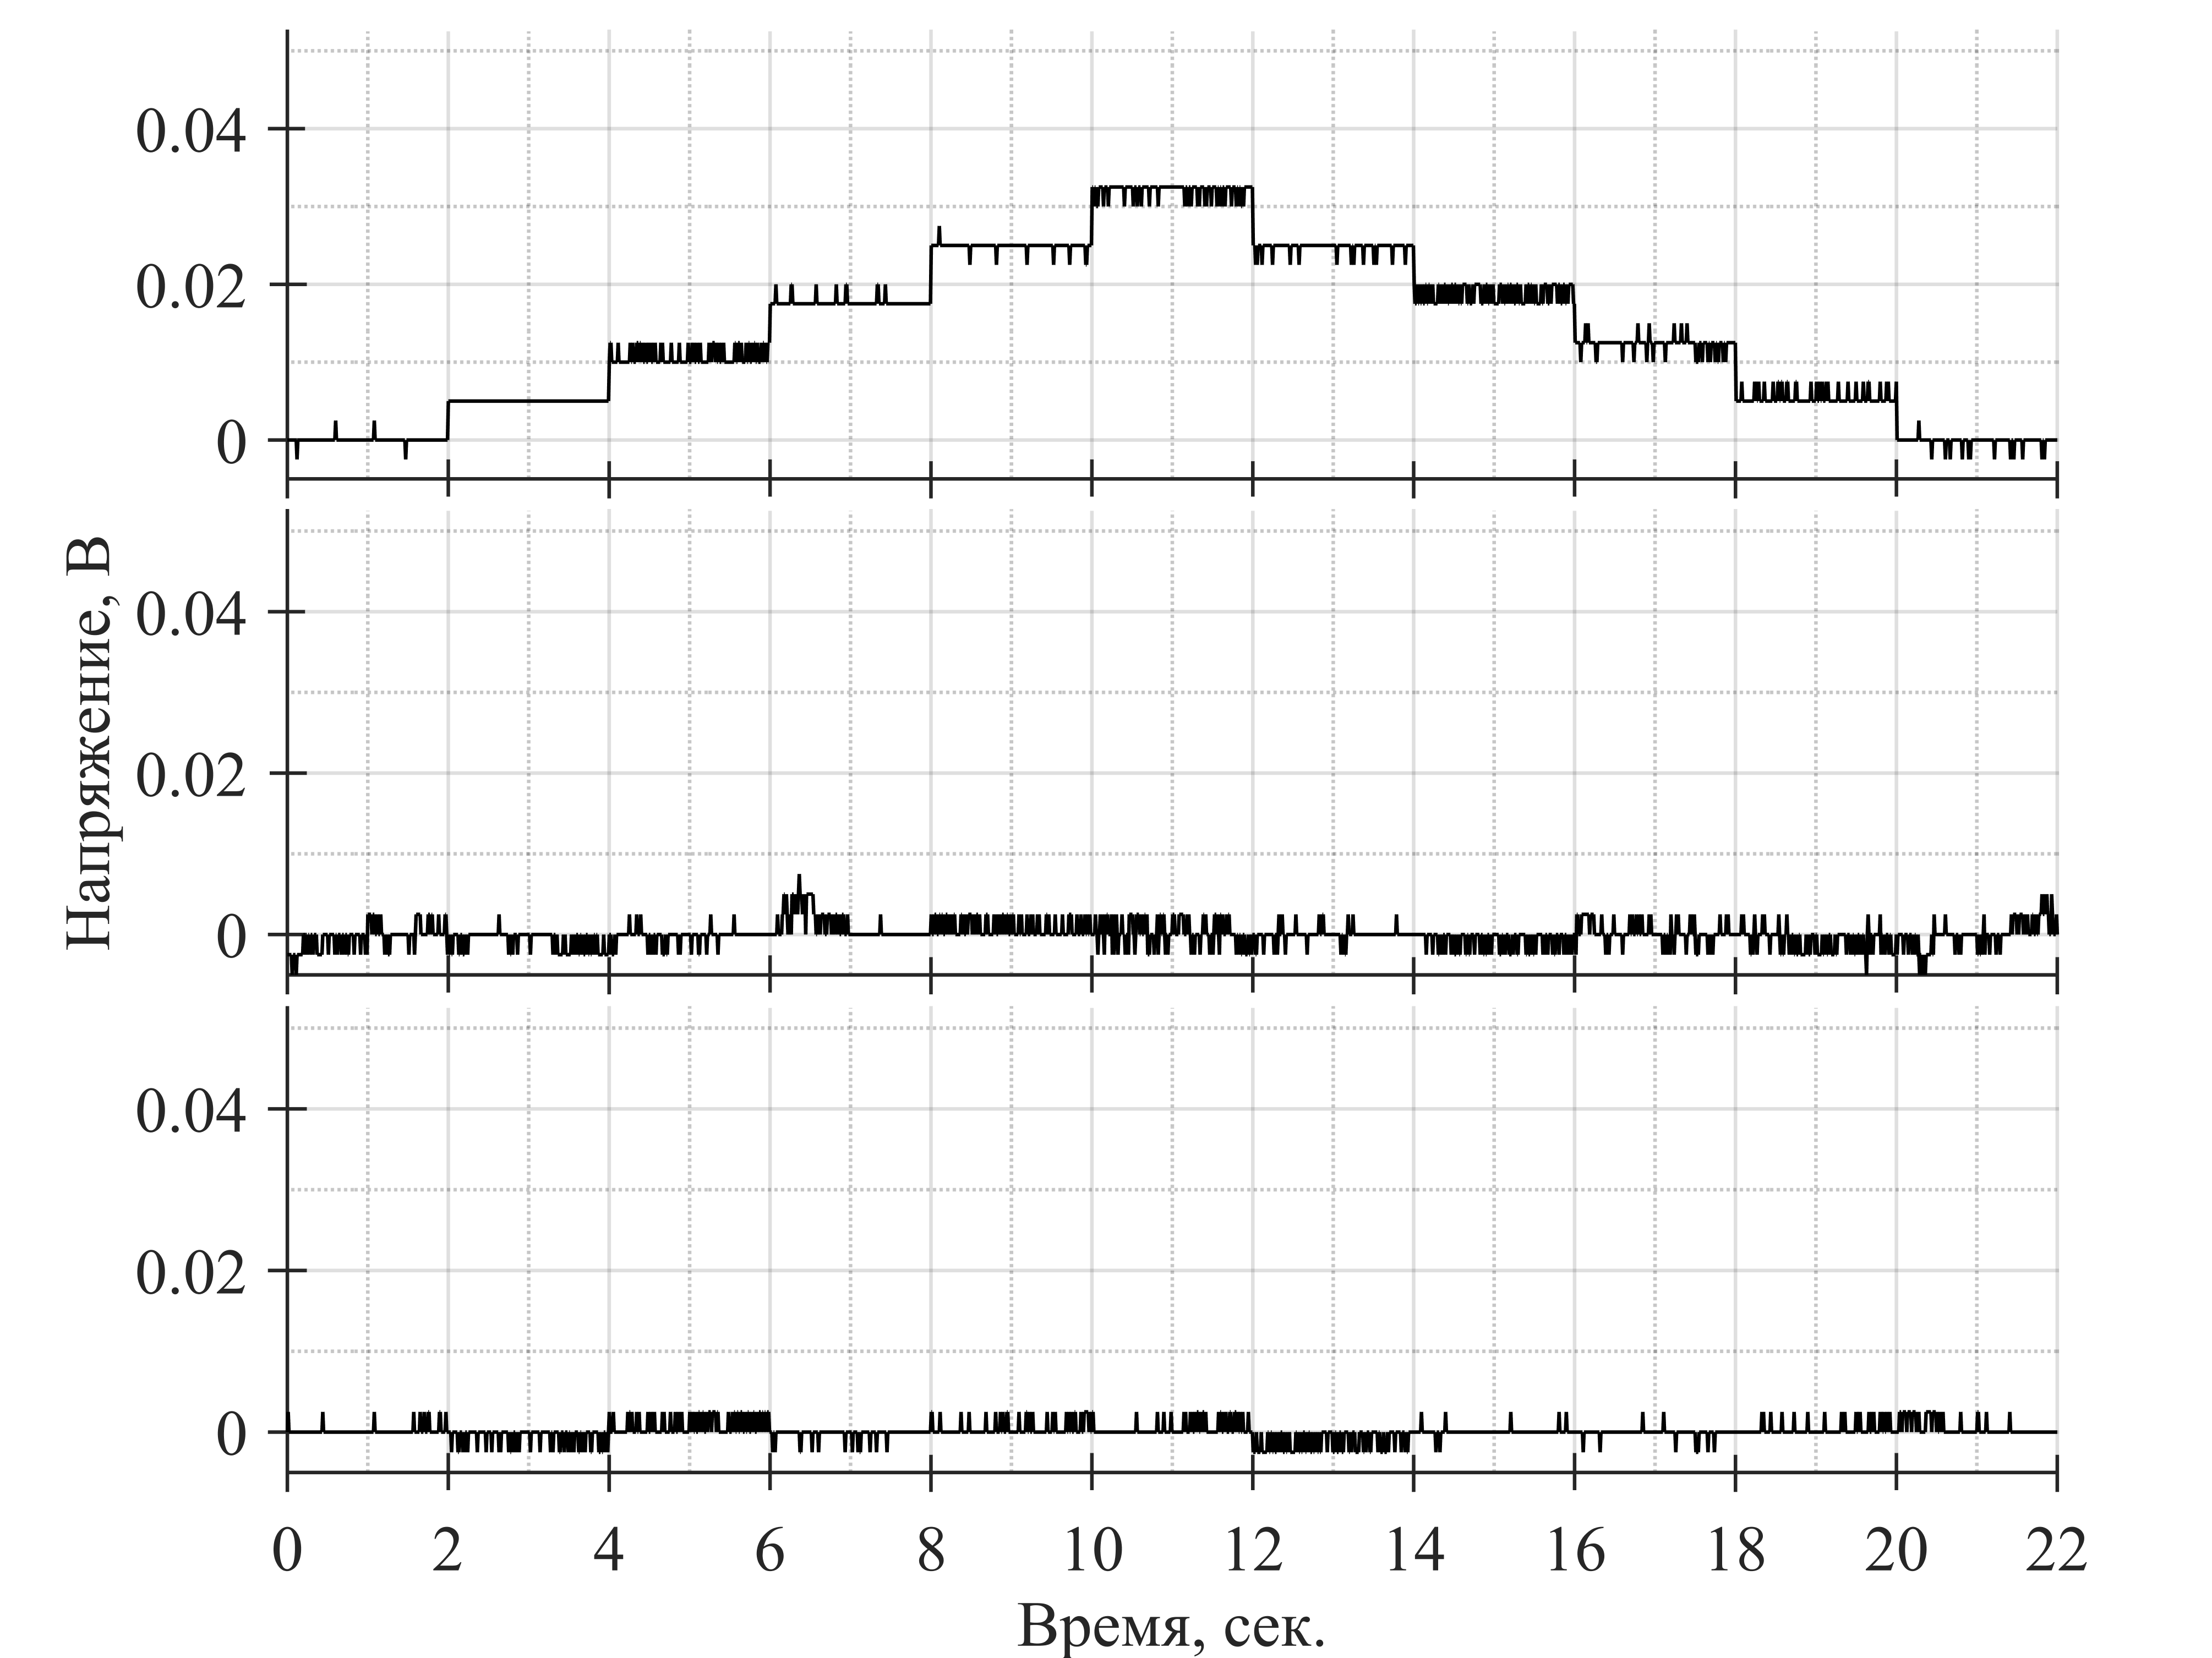
\includegraphics[width=0.7\textwidth]{CalibrationRawHor}
		
	% 	С веху вниз: горизонтальная, боковая, вертикальная составляющие усилия резания
	% 	\caption{Графики переходных процессов при тарировании горизонтальной составляющей усилия резания}  
	% 	\label{fig:CalibrationRawHor}  
	% \end{figure}
	
	% Используя данные с графиков переходных процессов можно получить зависимости изображенные на рисунке~\ref{fig:Calibration}. Из них видно что силы возникающие на тензометрическом звене имеют линейную зависимость от напряжения получаемого с тензометрических мостов. 

	% \begin{figure} [ht]
	% 	\centering
	% 	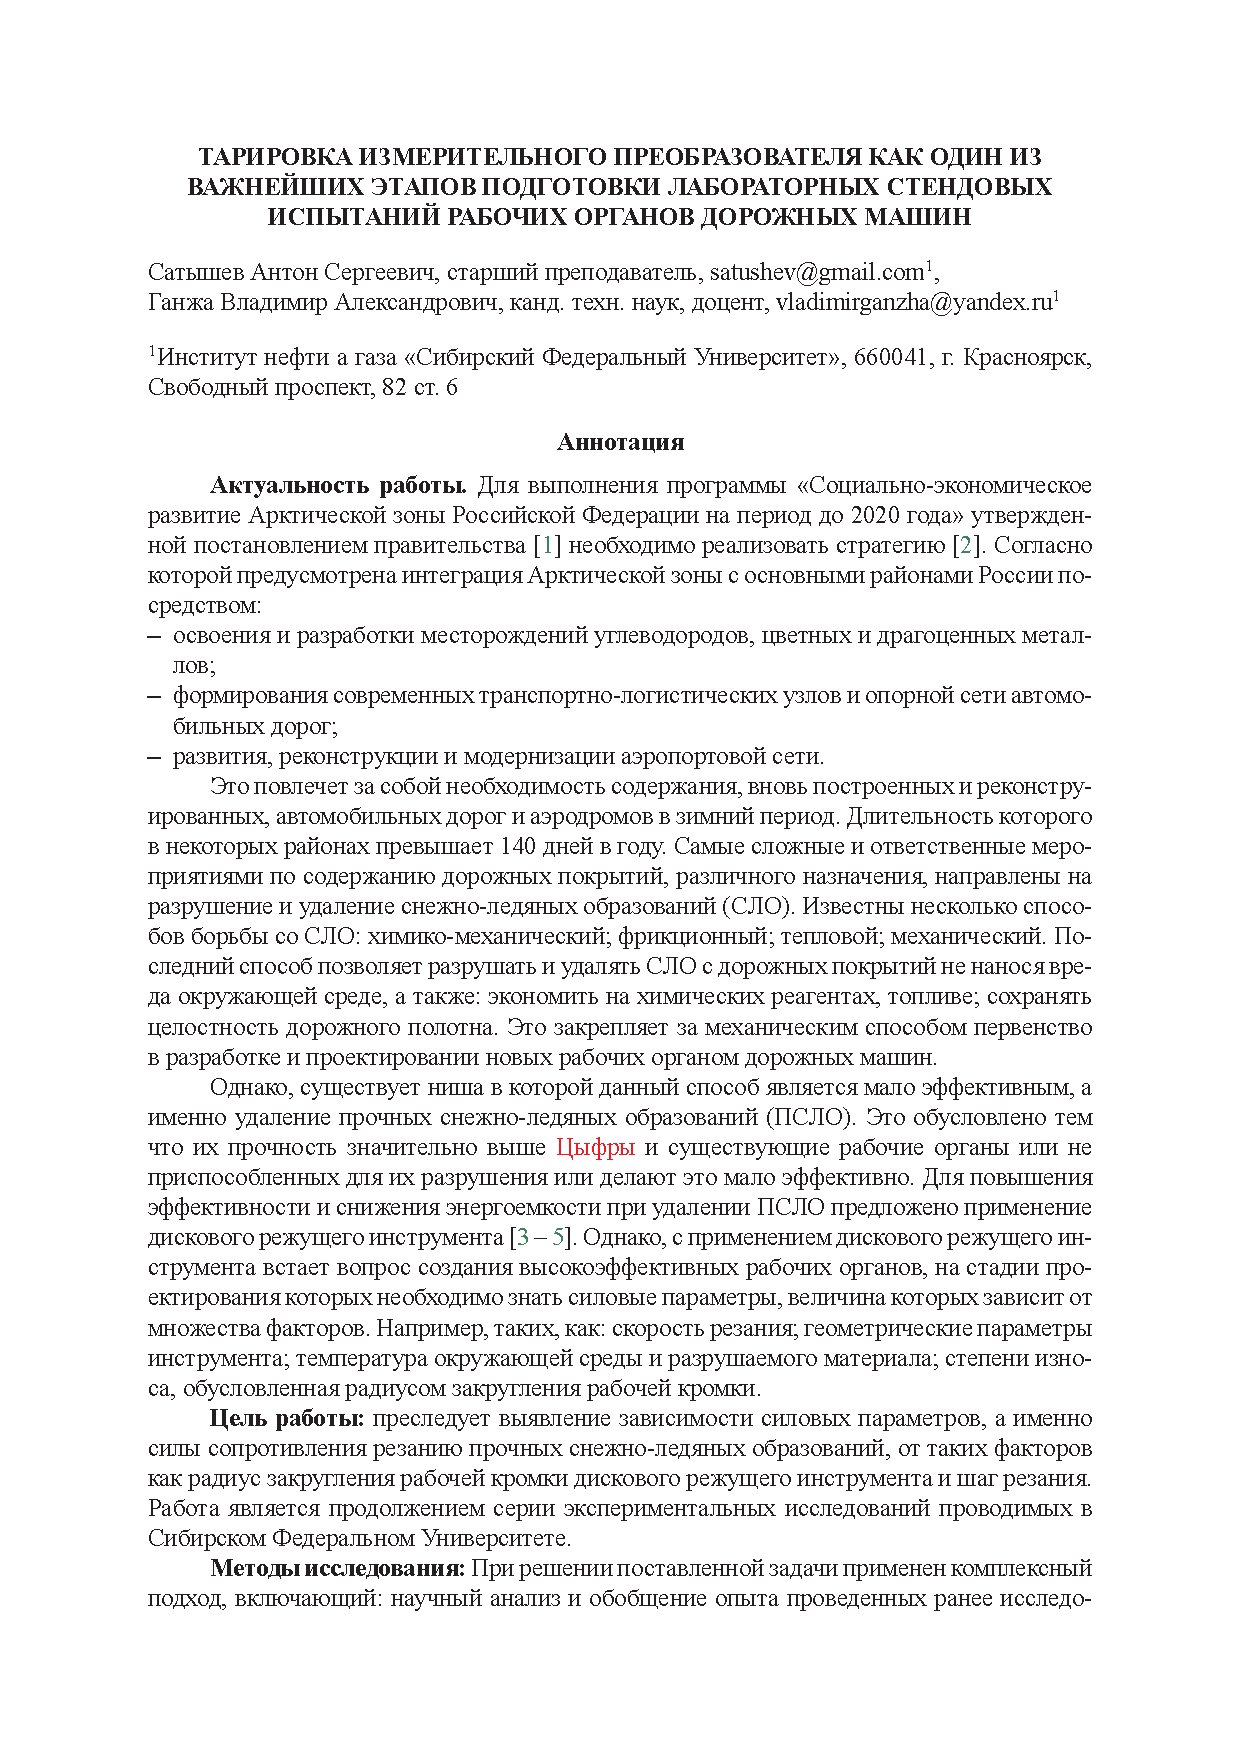
\includegraphics[width=0.7\textwidth]{Calibration}
		
	% 	1,2,3 "--- горизонтальная, бокова, вертикальная составляющие усилия резания соответственно при тарировании горизонтальной составляющей; 4,5,6 "--- аналогично  при тарировании боковой составляющей; 7,8,9 "--- аналогично при тарировании вертикальной составляющей.
	% 	\caption{Графики тарирования тензометрического звена}
	% 	\label{fig:Calibration}  
	% \end{figure}

	% Эти графики можно представить в виде уравнений:
	% \begin{align}
	% 	y_\text{гор}  & = 80074.568 \cdot x  \label{eq:TrendHor}\\
	% 	y_\text{бок}  & = 140953.396 \cdot x \label{eq:TrendLat}\\
	% 	y_\text{верт} & = 51338.284 \cdot x \label{eq:TrendVert}
	% \end{align}
	% Из уравнений \labelcref{eq:TrendHor,eq:TrendLat,eq:TrendVert} получим тарировочные коэффициенты: 8~0074.568~$ \slantfrac{\text{Н}}{\text{В}} $, 140~953.396~$ \slantfrac{\text{Н}}{\text{В}} $, 51~338.284~$ \slantfrac{\text{Н}}{\text{В}} $ для горизонтальной, боковой и вертикальной составляющей усилия резания соответственно.

	\section{Обработка результатов эксперимента}
	
	После проведения экспериментальных исследований влияния радиуса закругления рабочей кромки и шага резания на составляющие силы, возникающей на дисковом инструменте, при механическом разрушении льда, получен набор файлов с записью значений напряжений снятых с АЦП. Каждый файл соответствует своему сочетанию исследуемых параметров \textit{R} и \textit{t}. структура файла приведена на рисунке \ref{fig:FileMap}. Дальнейшее их использование предполагает обработку и оценку корректности методами математики и статистики, такими как:
	\begin{itemize}
		\item отброс грубых ошибок;   
		\item фильтрация:
		\item сглаживание;
		\item отброс постоянной составляющей;
		\item усреднение значений повторных экспериментов.
	\end{itemize}

	\begin{figure}[ht]
		\centering
		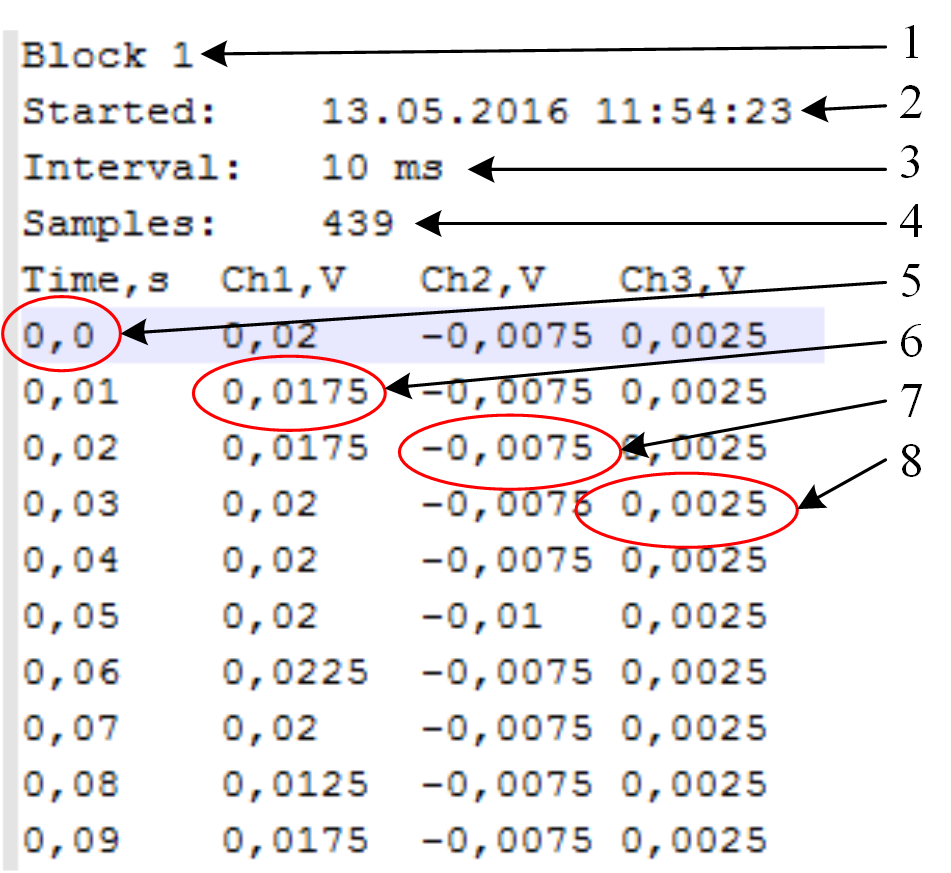
\includegraphics[width=0.6\textwidth]{DataFormat}

		1 "--- Название блока данных; 2 "--- Дата и время начала измерений; 3 "--- Интервал между измерениями в миллисекундах; 4 "--- Количество сохранённых измерений; 5 "--- Отсчёт времени в секундах; 6, 7, 8 "--- Значение напряжения на чувствительном элементе в вольтах для первого, второго и третьего канала соответственно
		\caption{Пример структуры файла хранения данных}
		\label{fig:FileMap}
	\end{figure}


	\subsection{Алгоритм отброса грубых ошибок}
	
	Для улучшения точности оценки переходного процесса и снижения влияния всевозможных внешних факторов целесообразно применить к полученному набору точек (сигналу) алгоритм отброса грубых ошибок \cite{LvovStat}.
	Суть алгоритма заключается в использовании метода максимального относительного отклонения:
	\begin{equation}\label{eq:MOO}
		\tau=\frac{|x_i-\bar{x}|}{\sigma_x},
	\end{equation} 
	где $ x_i $ "--- крайний (наибольший или наименьший) элемент сигнала; $ \bar{x} $ "--- среднее значение сигнала; $ \sigma_x $ "--- СКО сигнал.

	Сравнивая $ \tau $ с критическим значением $ \tau_{(p,n)} $, рассчитанным по формуле~\ref{eq:tau_krit}, можно сделать вывод является ли наблюдение грубой погрешностью или нет.
	\begin{equation}\label{eq:tau_krit}
		\tau_{(p,\ n)}=\frac{t_{(p,\ n-2)}\cdot\sqrt{n-1}}{\sqrt{n-2+|t_{(p,\ n-2)}|^2}}
	\end{equation}
	где $ t_{(p,\ n-2)} $ "--- критическое значение распределения Стьюдента при доверительной вероятность $ q=1-p $; $ n $ "--- количество наблюдений в сигнале переходного процесса.

	% Критическое значение распределения Стьюдента в ППП matlab можно вычислить с помощью функции \lstinline{tinv()}. 
	% \begin{lstlisting}
	% t = tinv(p / 100, n - 2);
	% \end{lstlisting}
	% где \lstinline{p} "--- вероятность; \lstinline{n} "--- количество наблюдений.

	Таким образом имеем алгоритм отброса грубых ошибок представленный на рисунке~\ref{fig:AlgDGE}.

	\begin{figure}[!ht]
		\centering
		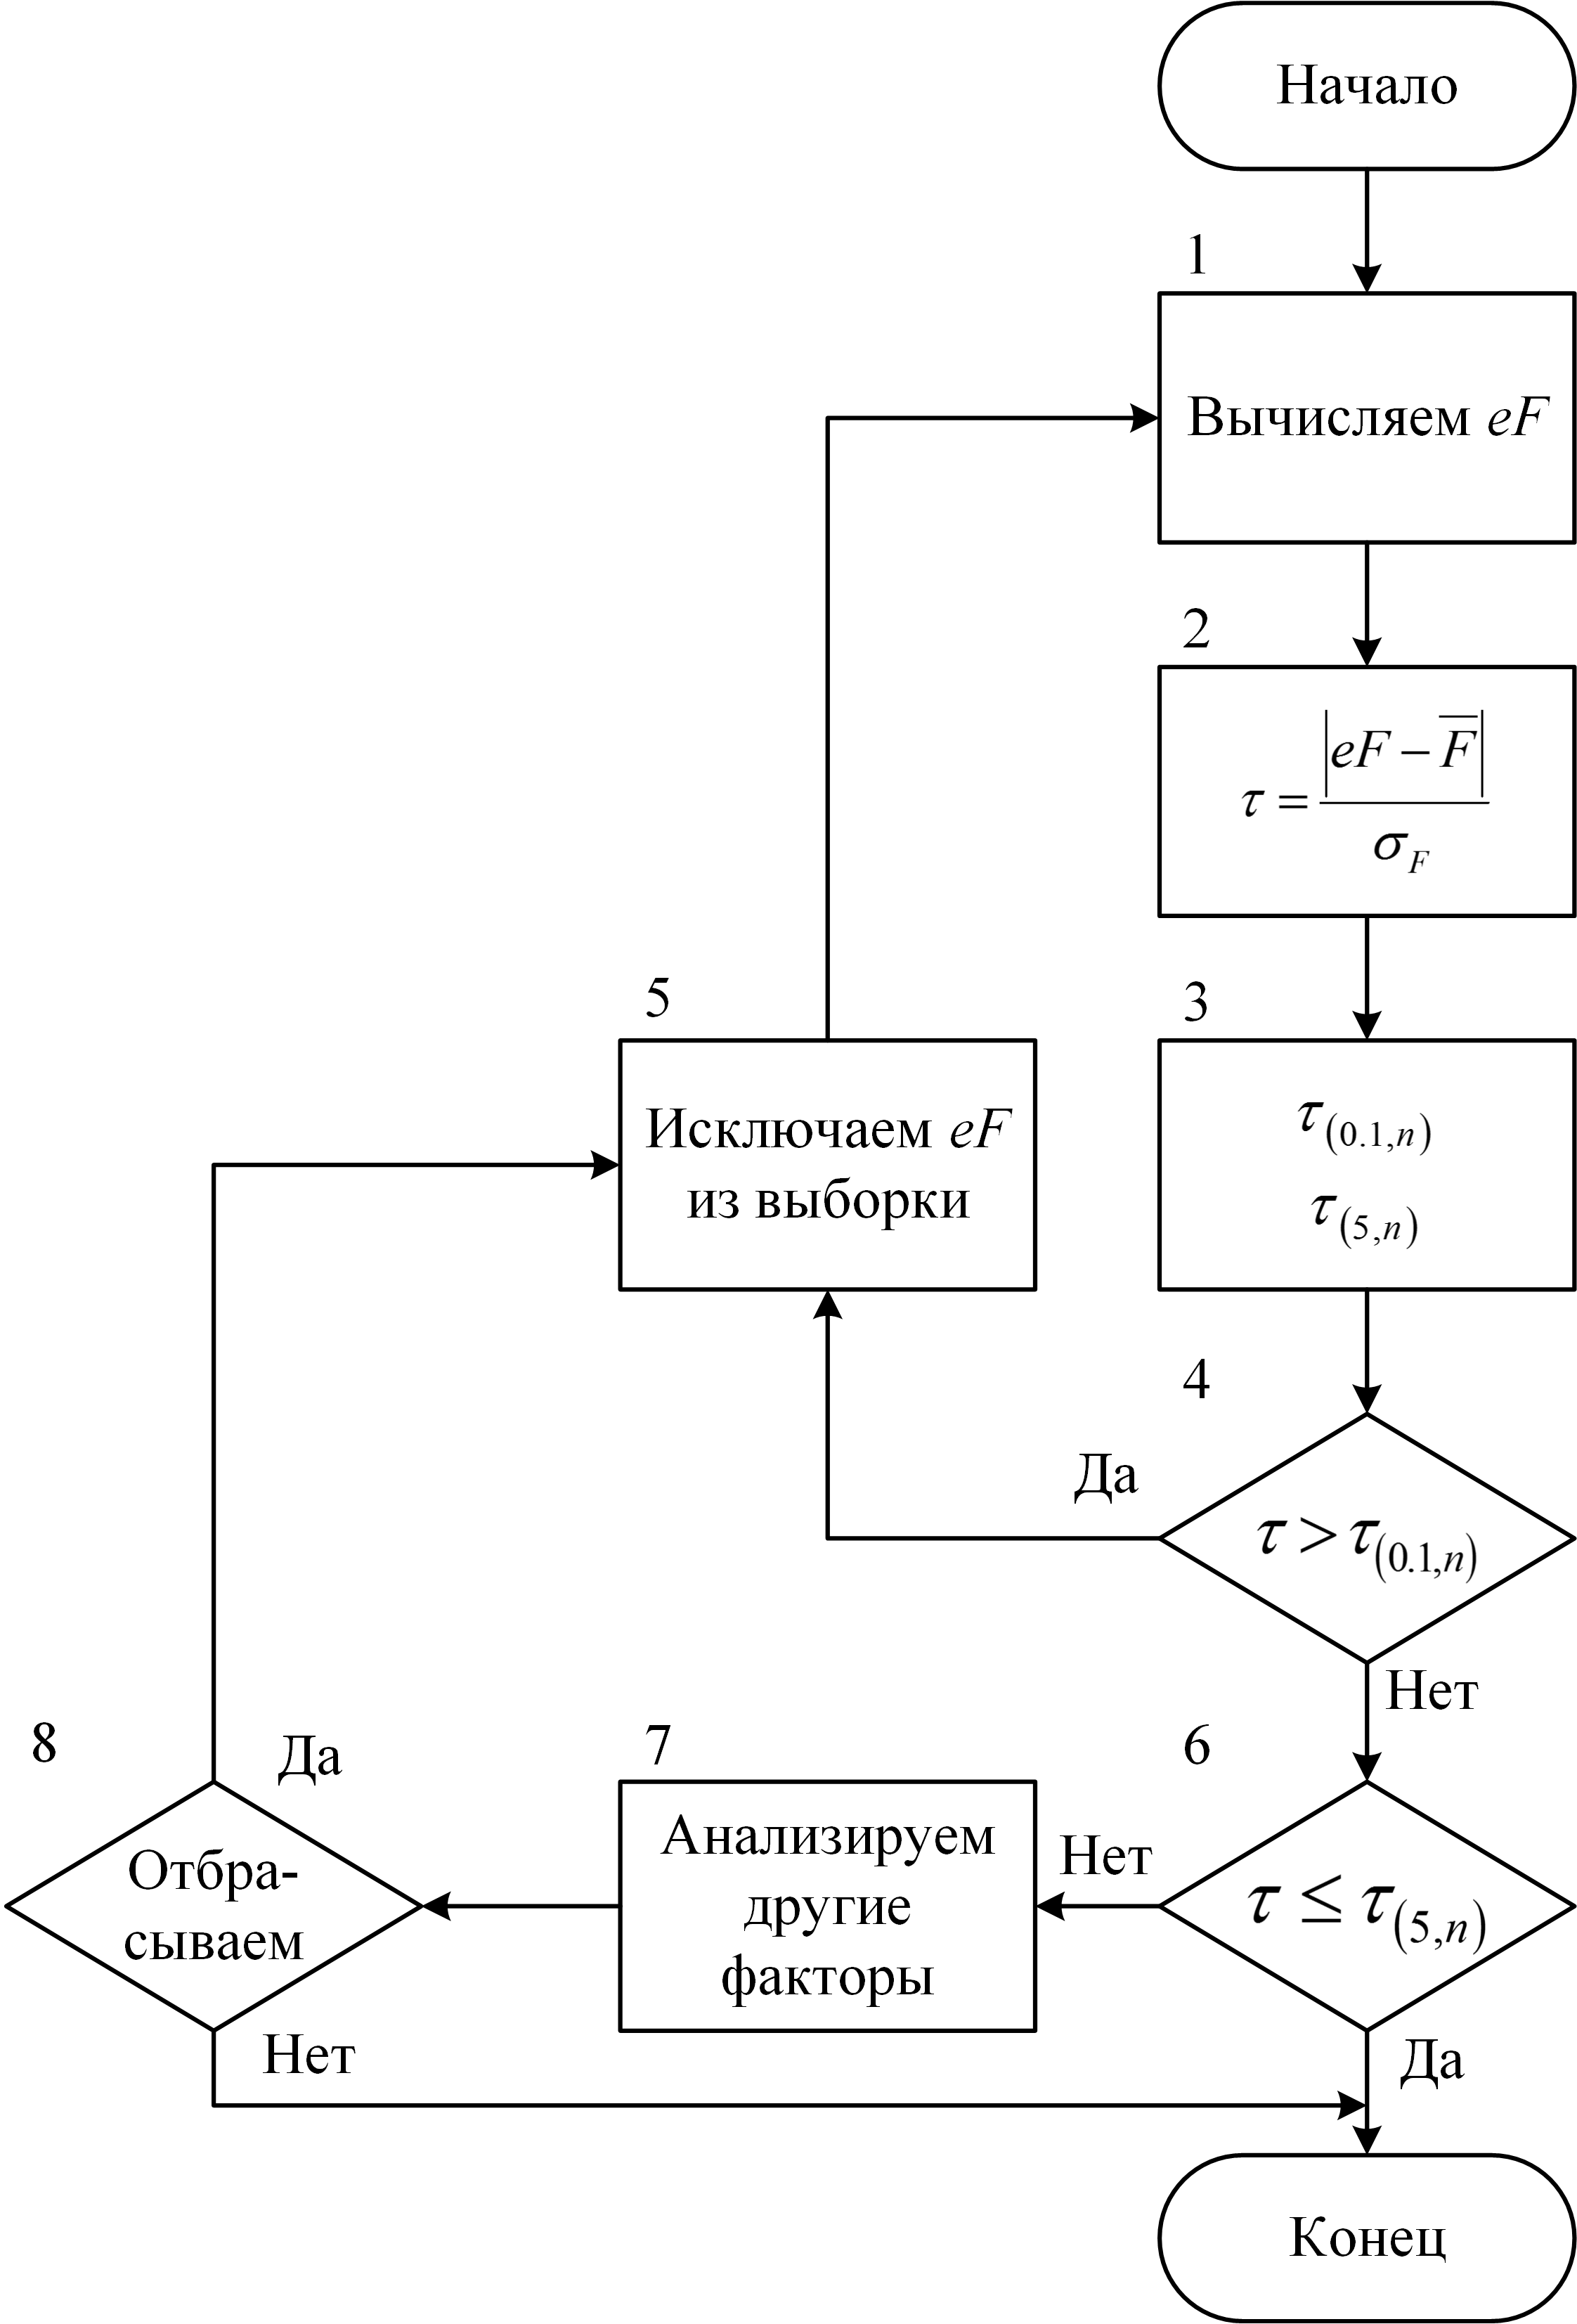
\includegraphics[scale=1]{images/DropGrossError}
		\caption{Алгоритм отброса грубых ошибок} 
		\label{fig:AlgDGE}  
	\end{figure}

	Имеет смысл ввести три группы наблюдений, удовлетворяющих следующим условиям:
	\begin{itemize}
		\item $ \tau \leqslant \tau_{(5\%,\ n)} $ нельзя отсеивать.
		\item $ \tau_{(5\%,\ n)} < \tau < \tau_{(0,1\%,\ n)} $ можно отсеять, если в пользу этой процедуры имеются и другие соображения.
		\item $ \tau > \tau_{(0,1\%,\ n)} $ отсеиваются всегда.
	\end{itemize}

	Приведем объяснение работы каждого блока в вербальном виде:
	\begin{enumerate}
		\item Из наблюдаемых значений выбирается максимальное и минимальное значение сигнала по модулю, далее значение сравниваются и выбирается наибольшее.\label{enum:alg_DGE_1}
		\item Рассчитывается $ \tau $ по формуле~\ref{eq:MOO}.
		\item Вычисляются критические точки $ \tau_{(0,1\%,\ n)} $ и $ \tau_{(5\%,\ n)} $ по формуле~\ref{eq:tau_krit}.
		\item Проверяется условие $ \tau > \tau_{(0,1\%,\ n)} $ если выполняется переходим к пункту~\ref{enum:alg_DGE_5}, иначе к~\ref{enum:alg_DGE_6}.
		\item Исключаем наблюдение из массива точек и переходим к пункту~\ref{enum:alg_DGE_1}.\label{enum:alg_DGE_5}
		\item Проверяем условие $ \tau \leqslant \tau_{(5\%,\ n)} $ если выполняется переходим к пункту~\ref{enum:alg_DGE_9}, иначе к~\ref{enum:alg_DGE_7}.\label{enum:alg_DGE_6}
		\item Анализируем другие факторы способные указать на допущение грубой ошибки.\label{enum:alg_DGE_7}
		\item Принимаем решение отбрасывать или нет. Если отбрасываем переходим к пункту~\ref{enum:alg_DGE_5}, иначе к~\ref{enum:alg_DGE_9}.\label{enum:alg_DGE_8}
		\item Выход из алгоритма. Оставшиеся наблюдения и есть полезный сигнал.\label{enum:alg_DGE_9}
	\end{enumerate}

	\subsection{Сглаживание сигнала}
	
	Для более наглядной читаемости и устранения влияния высокочастотных помех, предлагается применение цифрового фильтра <<Скользящая средняя>>. Этот способ является наиболее простым в реализации и даёт хорошие результаты при правильном подборе апертуры. Скользящее среднее (moving average \textbf{MA}) вычисляется по формуле:

	\begin{equation}
		\begin{multlined}
			MA_t=\frac{1}{n}\sum_{i=0}^{n-1}\left( b_i \cdot p_{t-i}\right) = \\
			= b_0 \cdot p_t+b_1 \cdot p_{t-1}+\cdots+b_i \cdot p_{t-i}+\cdots+b_{n-2} \cdot p_{t-n-2}+b_{n-1} \cdot p_{t-n-1},
		\end{multlined}
	\end{equation}
	где $ MA_t $ "--- значение скользящего среднего в точке $ t $; $ n $ "--- количество значений исходной функции для расчёта скользящего среднего (апертура); $ p_{t-i} $ "--- значение исходной функции в точке $ t-i $; $ b_i $ "--- вектор весовых коэффициентов.
	
	Обычно для фильтров скользящего среднего применяется равномерное распределение весов. Например, если $ n = 4 $, то $ b = \left[ \frac{1}{4}\ \frac{1}{4}\ \frac{1}{4}\ \frac{1}{4}\right] $. Такой фильтр будет называться простым скользящим средним (simple moving average SMA).
	В данной работе предлагается выбирать весовые коэффициенты для MA путём оценки автокорреляционной функции от требуемого сигнала. На рисунке~\ref{fig:Autocorr} построена автокорреляционная функция и ее доверительные интервалы $ [-0.09623\ 0.09623] $. Предлагается за весовые коэффициенты взять первые значения автокорреляционной функции, до пересечения её и <<верхней>> доверительной границы.

	\begin{figure}[ht] 
		\centering
		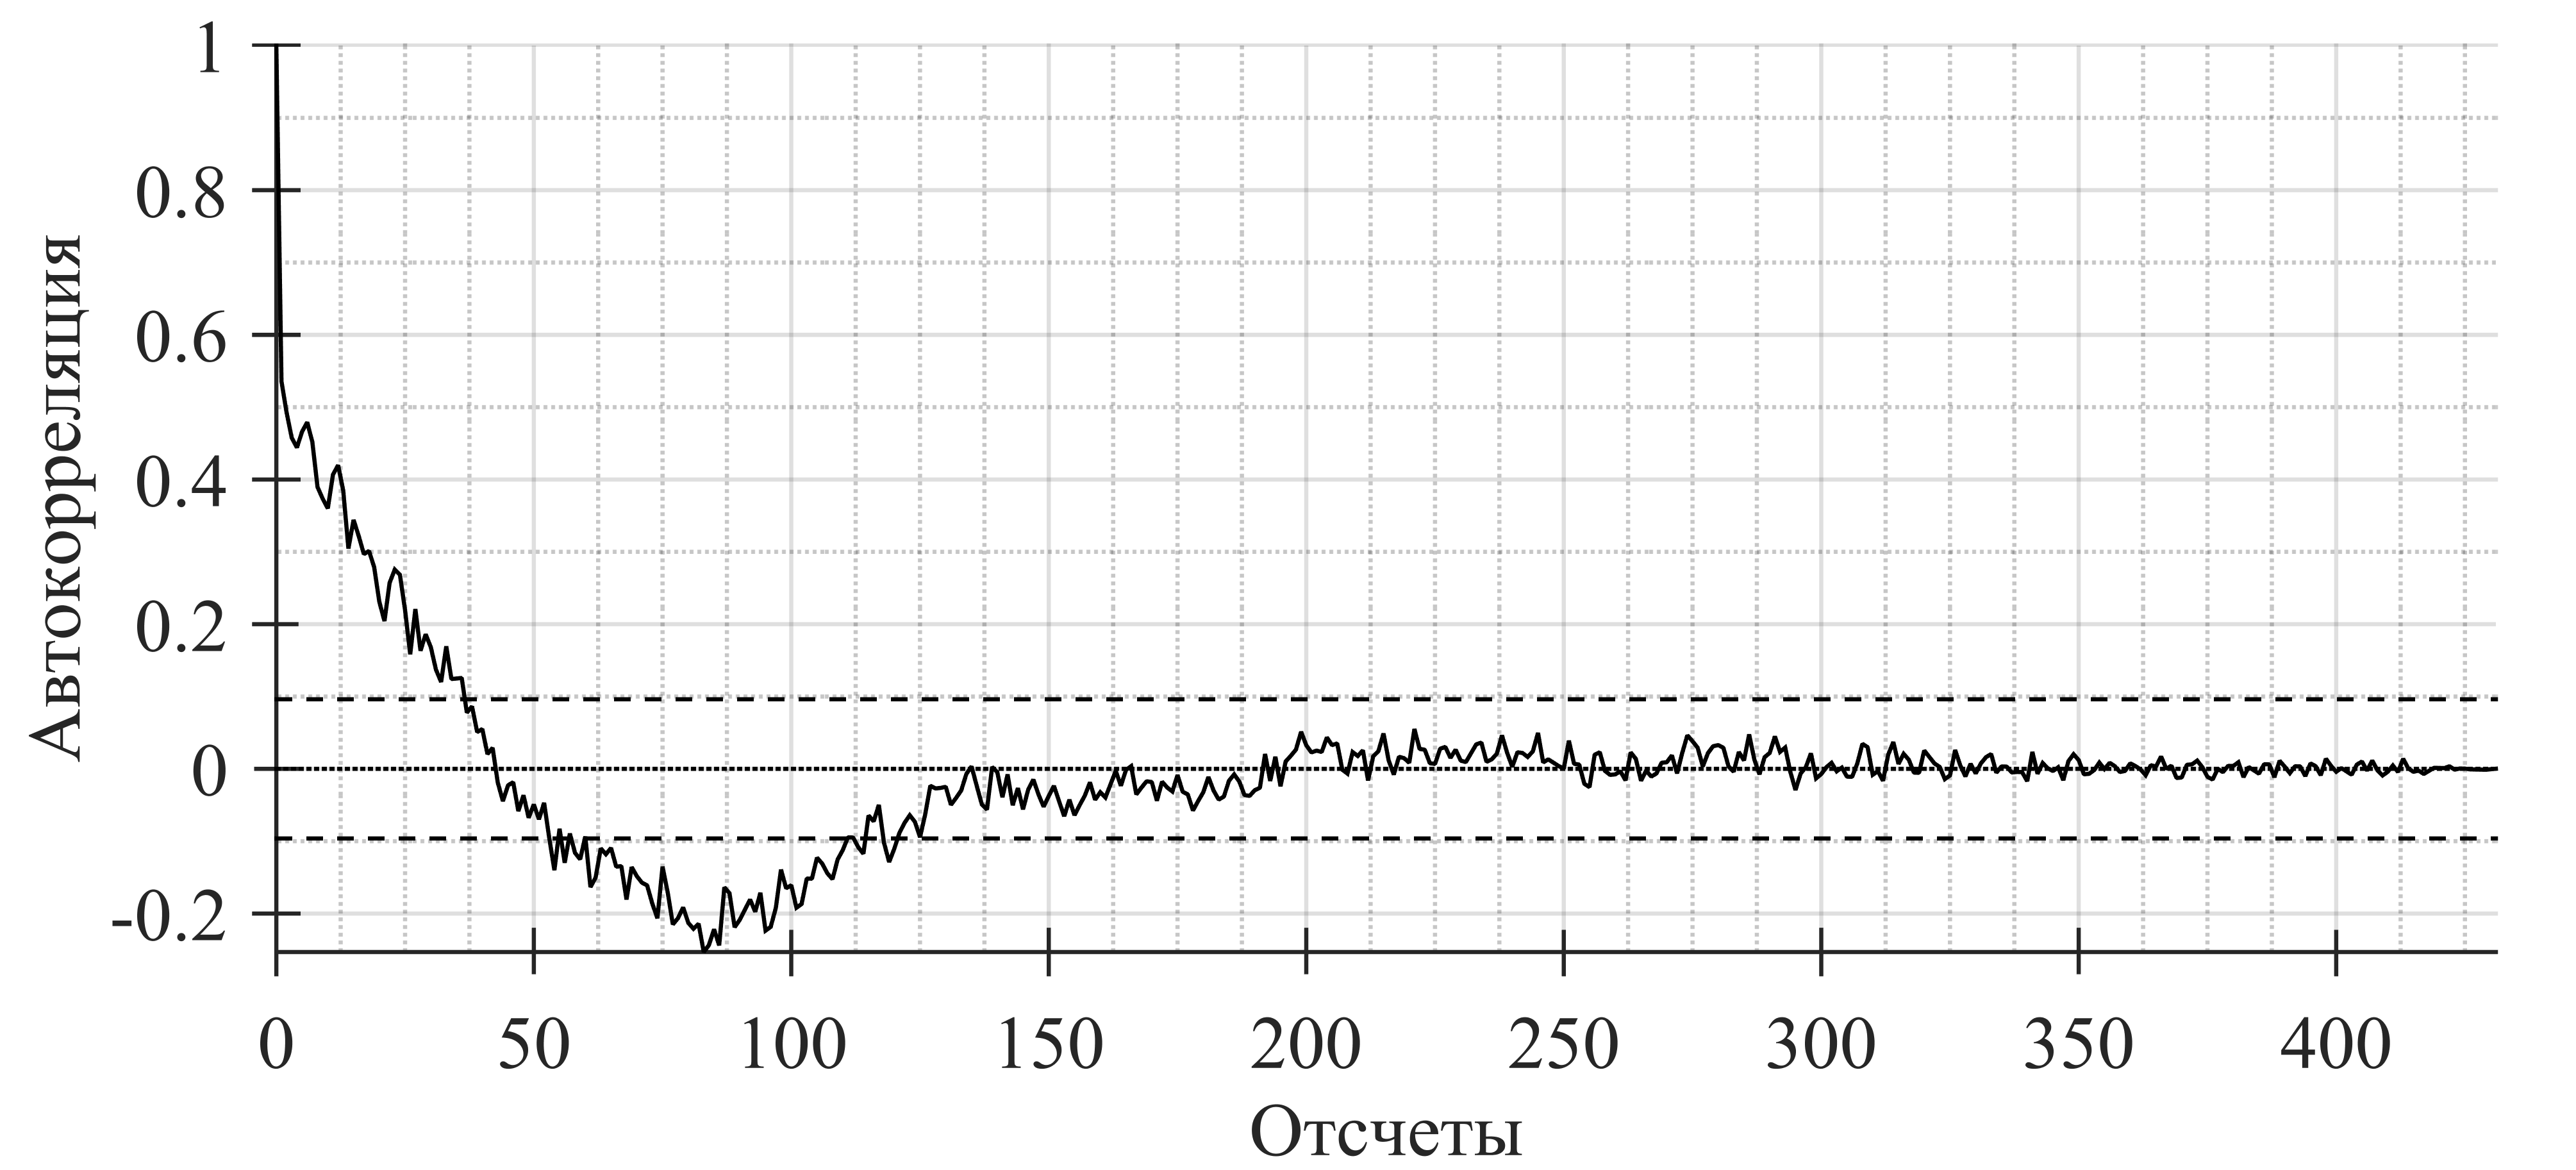
\includegraphics[width=0.8\textwidth]{Autocorr}
		\caption{Автокорреляционная функция с доверительным интервалом} 
		\label{fig:Autocorr}  
	\end{figure}

	Такой алгоритм обусловлен включением в окно скользящего среднего только <<тесно>> связанных между собой значений целевой функции, и в тоже время применяет веса к включённым значениям согласно их влиянию.

	\section{Заключение}

	\begin{figure}[ht] 
		\centering
		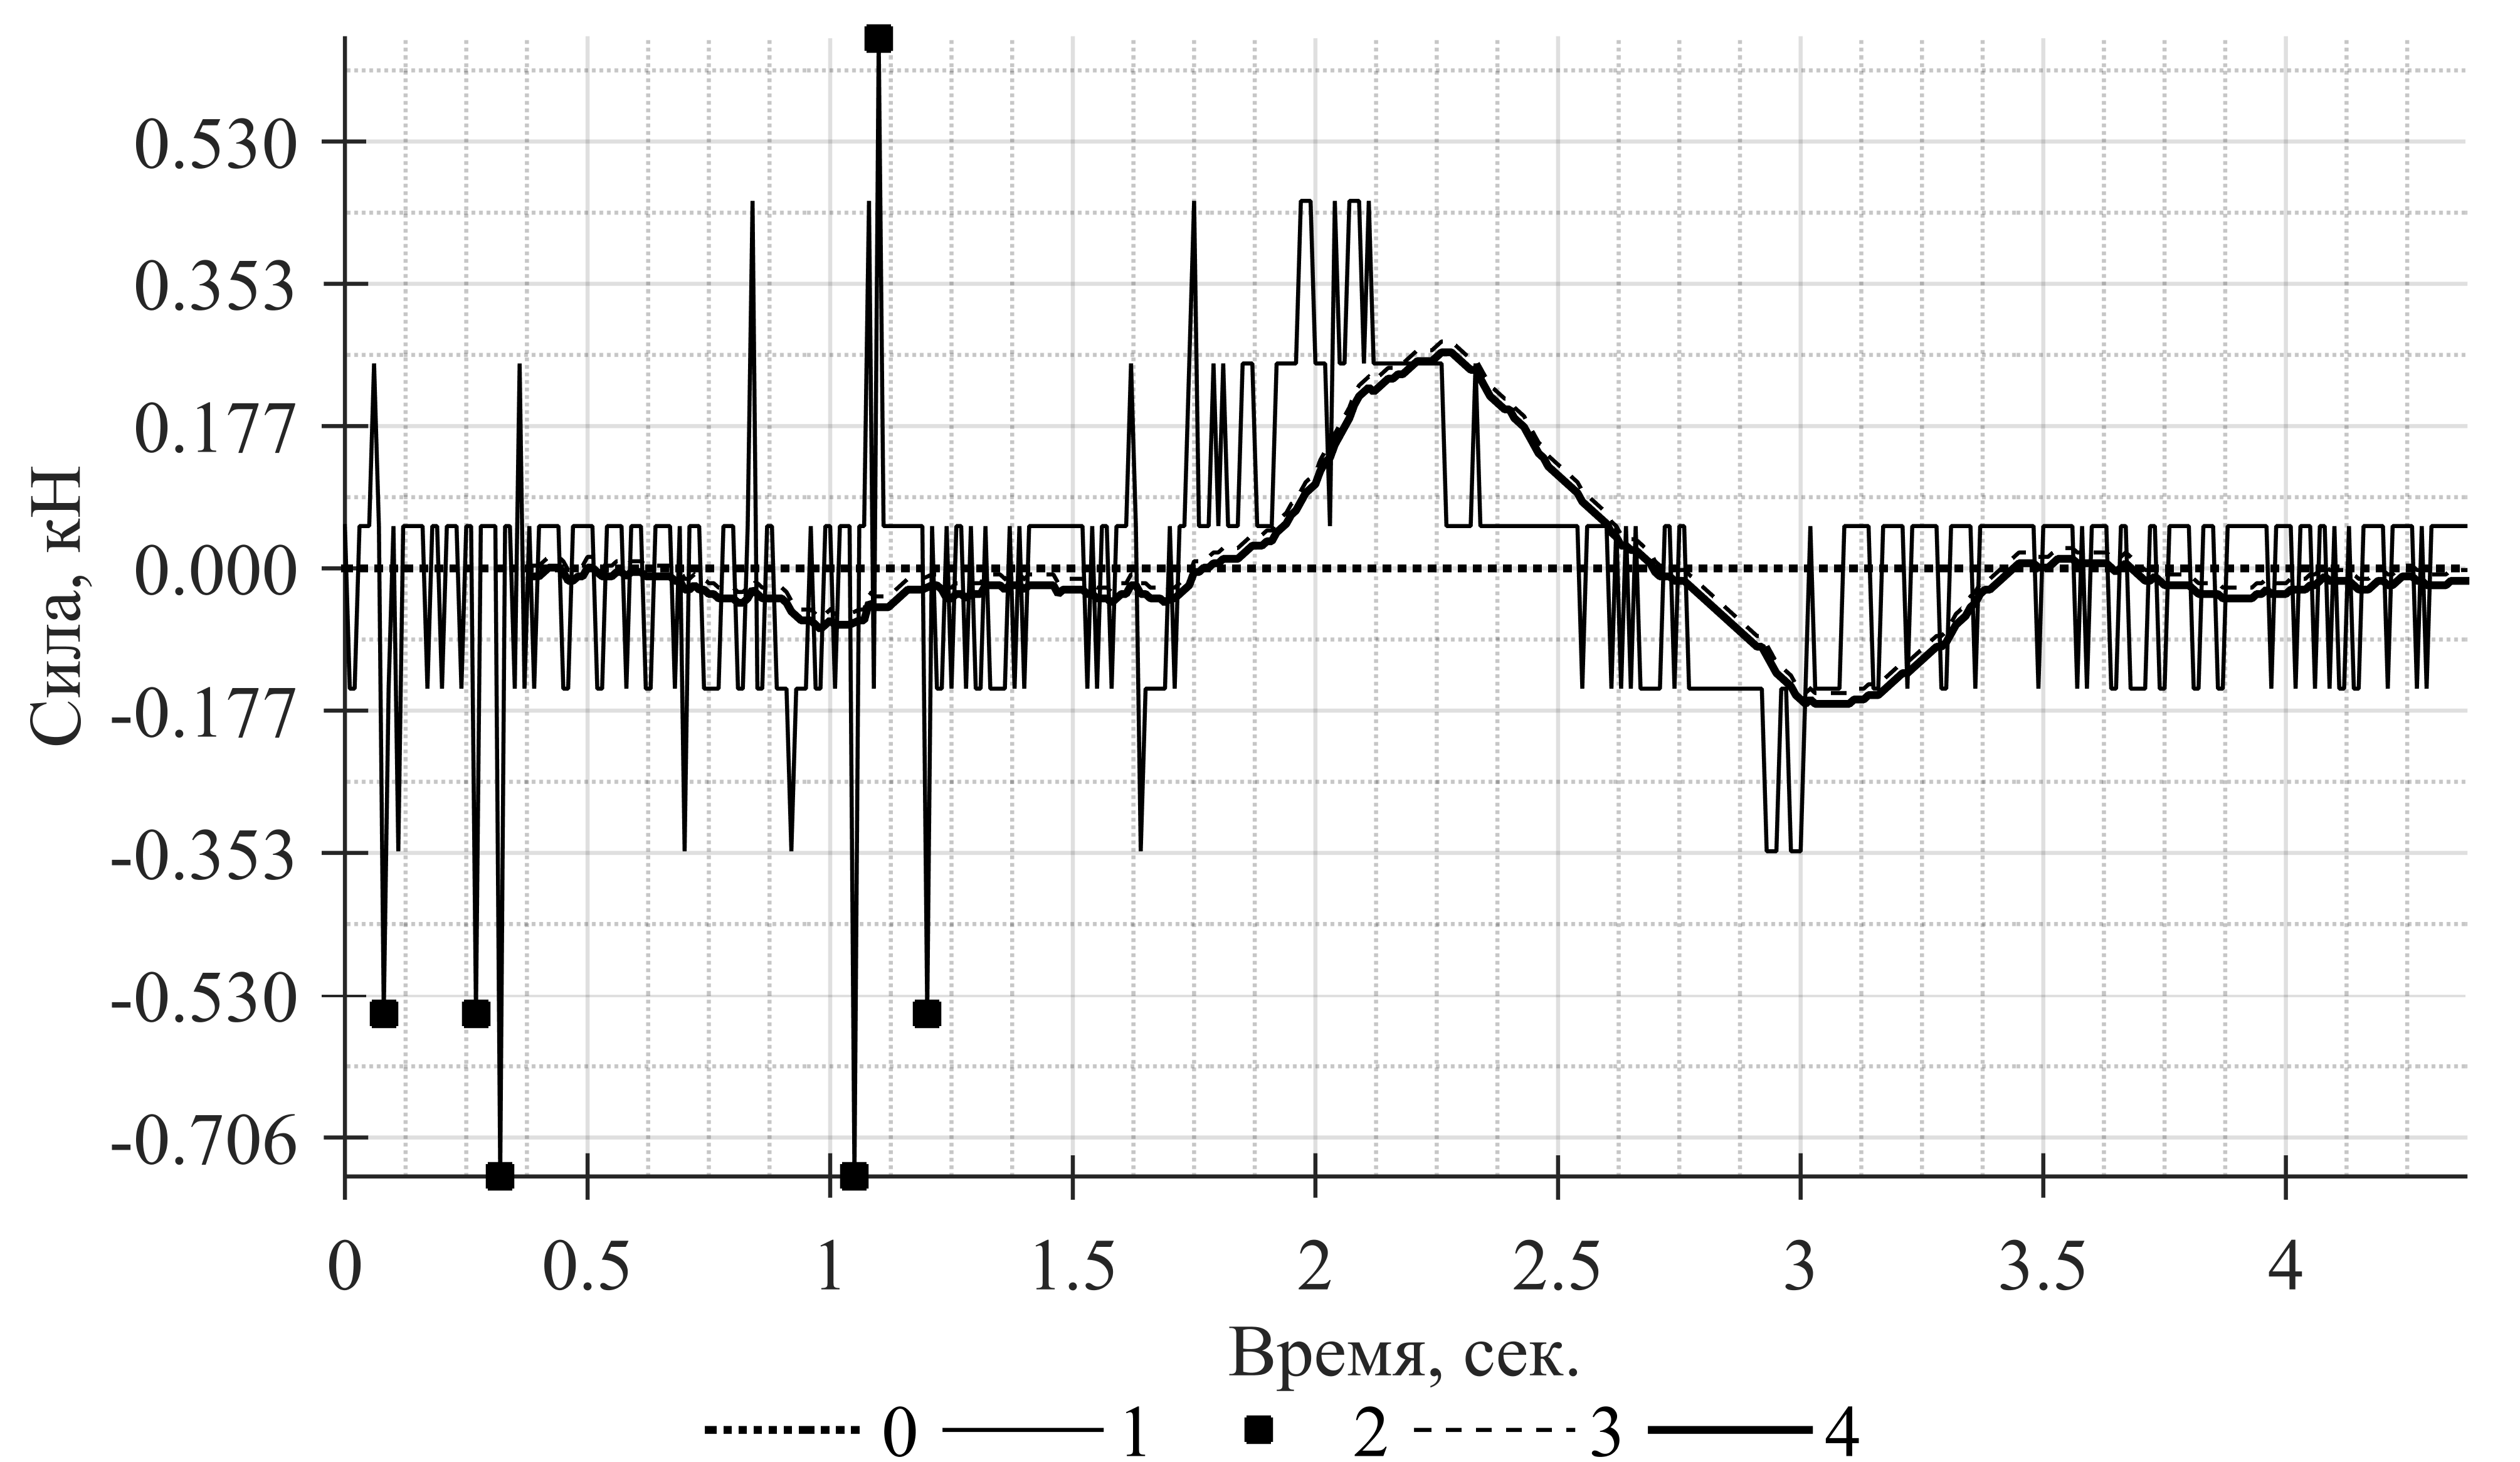
\includegraphics[width=1\textwidth]{SignalRaw}
		
		1 "--- сигнал полученный с АЦП <<сырой>>; 2 "--- отброшенные точки в результате работы алгоритма отброса грубых ошибок; 3 "--- результат скользящего среднего; 4 "--- результат отброса постоянной составляющей.
		\caption{Переходный процесса разрушения льда} 
		\label{fig:SignalRaw}  
	\end{figure}

	Анализируя работу описанных алгоритмов, по рисунку \ref{fig:SignalRaw} можно видеть отброшенные пиковые выбросы сигнала 2, рассчитанные с помощью алгоритма отброса грубых ошибок. Такие выбросы могут свидетельствовать о кратковременных скачках напряжения в питающей сети, обусловленных работой силового оборудования, такого как трехфазный двигатель привода лабораторного стенда, холодильная установка.

	Так же на графике представлен сглаженный сигнал переходного процесса резания льда 3, полученный путем применения алгоритма скользящего среднего с адаптивным окном сглаживания. Как видно график 3 имеет некоторое смещение по временной оси, которое обусловлено размером окна сглаживания. Смещение не является критичны, так как расположено в начале временной оси, в тот момент времени когда, происходит движение резца в свободной состоянии (до момента внедрения в ледяной массив). Так же на графике 3 явно видны отрицательные значения сигнала. Отрицательные значения на временном промежутке от 0,375 до 1,75 секунд объясняются наличием упругих элементов в тензометрическом звене и не нулевыми моментами инерции кронштейна и дискового режущего инструмента. Отрицательные значения на промежутке времени с 2,75 по 3,5 секунд имеют тот же характер, однако, обусловлены резкой остановкой тензометрической головки вместе с оснасткой и инструментом.

	График 4 мало отличается от графика 3, однако, это сигнал имеющий нулевую постоянную составляющую. Столь малые отличия объясняются хорошей подстройкой переменного резистора в мостовой схеме включения тензометрических резисторов. Однако, такая подстройка не редко может производиться не точно или вообще не производится. Поэтому для получения результирующего сигнала используется алгоритм отброса постоянной составляющей. А именно, перевод сигнала в частотную область и вычисления амплитуды нулевой частоты.

	Таким образом полученные данные становятся более читаемыми и пригодными к дальнейшему анализу, которы подразумевает под собой построении математической модели взаимодействия дискового режущего инструмента с ПСЛО, которая будет учитывать такие параметры как радиус закругления рабочей кромки и шаг резания.